\documentclass[border=10pt]{standalone}
\usepackage{tikz}\usepackage{amsmath}\usetikzlibrary{arrows.meta}
\begin{document}
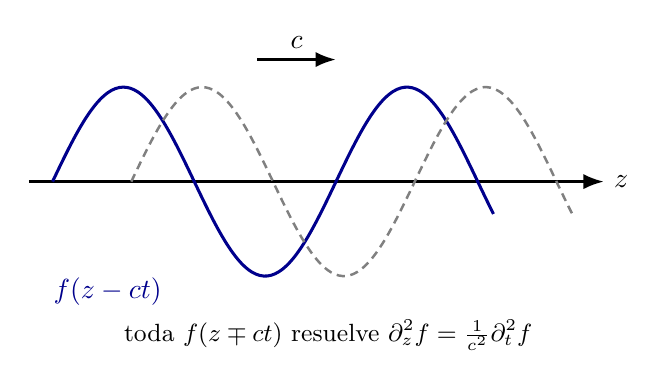
\begin{tikzpicture}[line width=0.9pt,>={Latex[length=2.6mm]}]
  \draw[->] (-0.3,0)--(7,0) node[right]{$z$};
  \draw[blue!55!black,line width=1.1pt,domain=0:5.6,samples=120,smooth] plot (\x,{1.2*sin(\x*100)});
  \draw[gray,densely dashed,domain=1:6.6,samples=120,smooth] plot (\x,{1.2*sin((\x-1)*100)});
  \draw[->,line width=1.1pt] (2.6,1.55)--(3.6,1.55) node[midway,above]{$c$};
  \node[blue!55!black] at (0.7,-1.4){$f(z-ct)$};
  \node at (3.5,-1.95){\small toda $f(z\mp ct)$ resuelve $\partial_z^2 f=\tfrac{1}{c^2}\partial_t^2 f$};
\end{tikzpicture}
\end{document}
